\chapter{从传统虚拟化到虚拟容器}
\label{cha:virtualization-and-container}

虚拟化技术从 2008 开始越来越热,到了今天,已经成为了企业 IT 技术中必不可少的了。
本章节首先介绍虚拟化技术的演变以及在发展过程中产生的几种类型,然后介绍几种用户
层 (user-land) 的虚拟化管理工具,然后介绍本次实验采用的宿主系统 CentOS 7 的
一些特性,最后罗列 OpenStack 支持的几种虚拟化方案。

在下文中,如果没有特殊说明,用虚拟机管理程序指代 hypervisor ,用宿主机
指代 host ,也就是承载虚拟机管理程序的物理机器和上面运行的操作系统,用
客户机或者客户虚拟机指代 guest ,也就是运行在宿主机上由虚拟机管理程序
模拟出的环境上的宾客操作系统及相关软件。

\section{虚拟化技术的演变}

和其它大多数技术一样,虚拟化技术也不是一蹴而就的,它经历了以下几种形态的演变和发展
~\cite{deep-into-kvm}:

\subsection{软件模拟}

严格来说,模拟器 (emulator) 不是一种虚拟化方式,但是它也可以实现在宿主机上
运行不同的客户机操作系统。它的出现早于虚拟化技术,而且实现的方式形形色色,例如
早期的 Macintosh 电脑可以安装兼容 DOS 系统的扩展卡,从而运行为 PC 编写的
程序。现在常见的形式是软件模拟,例如 QEMU \footnote{QEMU 可以和 KVM 配合,
工作在 virtualizer 模式,在这里只讨论 emulator 模式}。

\begin{figure}[h]
    \centering
    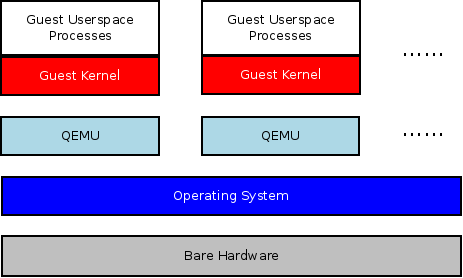
\includegraphics[width=0.7\textwidth]{qemu-arch}
    \caption{QEMU 的基本结构}
\end{figure}

和 Bochs 不同,QEMU 不仅能模拟 X86 架构的处理器,还能支持 ARM / MIPS / PowerPC
 / Sparc / Xtensa 等多种架构的处理器。而且 QEMU 和 Valgrind 一样使用的是动态翻译。
所谓静态翻译,就是不需要执行程序本身,一次读入整个二进制文件,完成翻译;所谓动态翻译,
就是在执行过程中只看一小段程序,比如一个基本块 (basic block) ,然后翻译并缓存 (caching)
翻译好的目标代码。这样的好处是二进制程序只在需要的时候被翻译,比如一个循环,执行一次之后
又跳转回到和一开始相同的代码,那么只需要指向缓存中已经翻译好的代码就可以了,而不用
重新翻译一遍。

当然 Valgrind 本质上是一个检查内存错误的 memcheck 工具,这是它和 QEMU 根本上的不同。
如果模拟器工作在纯软件模拟,执行效率是不高的,但是好处是理论上可以模拟任何硬件,
以至于不存在的硬件。

\subsection{虚拟化层翻译}

\section{管理工具}

\section{RedHat 和 CentOS 7}

\section{OpenStack 支持的虚拟化技术}
